
\section{Benutzerhandbuch}

\subsection{Projektauswahlfenster}
Das Programm startet mit einem Auswahlfenster für Projekte. Hier haben Sie die Möglichkeit zuletzt erstellte Projekte zu öffnen, andere existierende Projekte hinzuzufügen oder ein neues Projekt zu erstellen. 

\begin{figure}[h!]
	\centering
	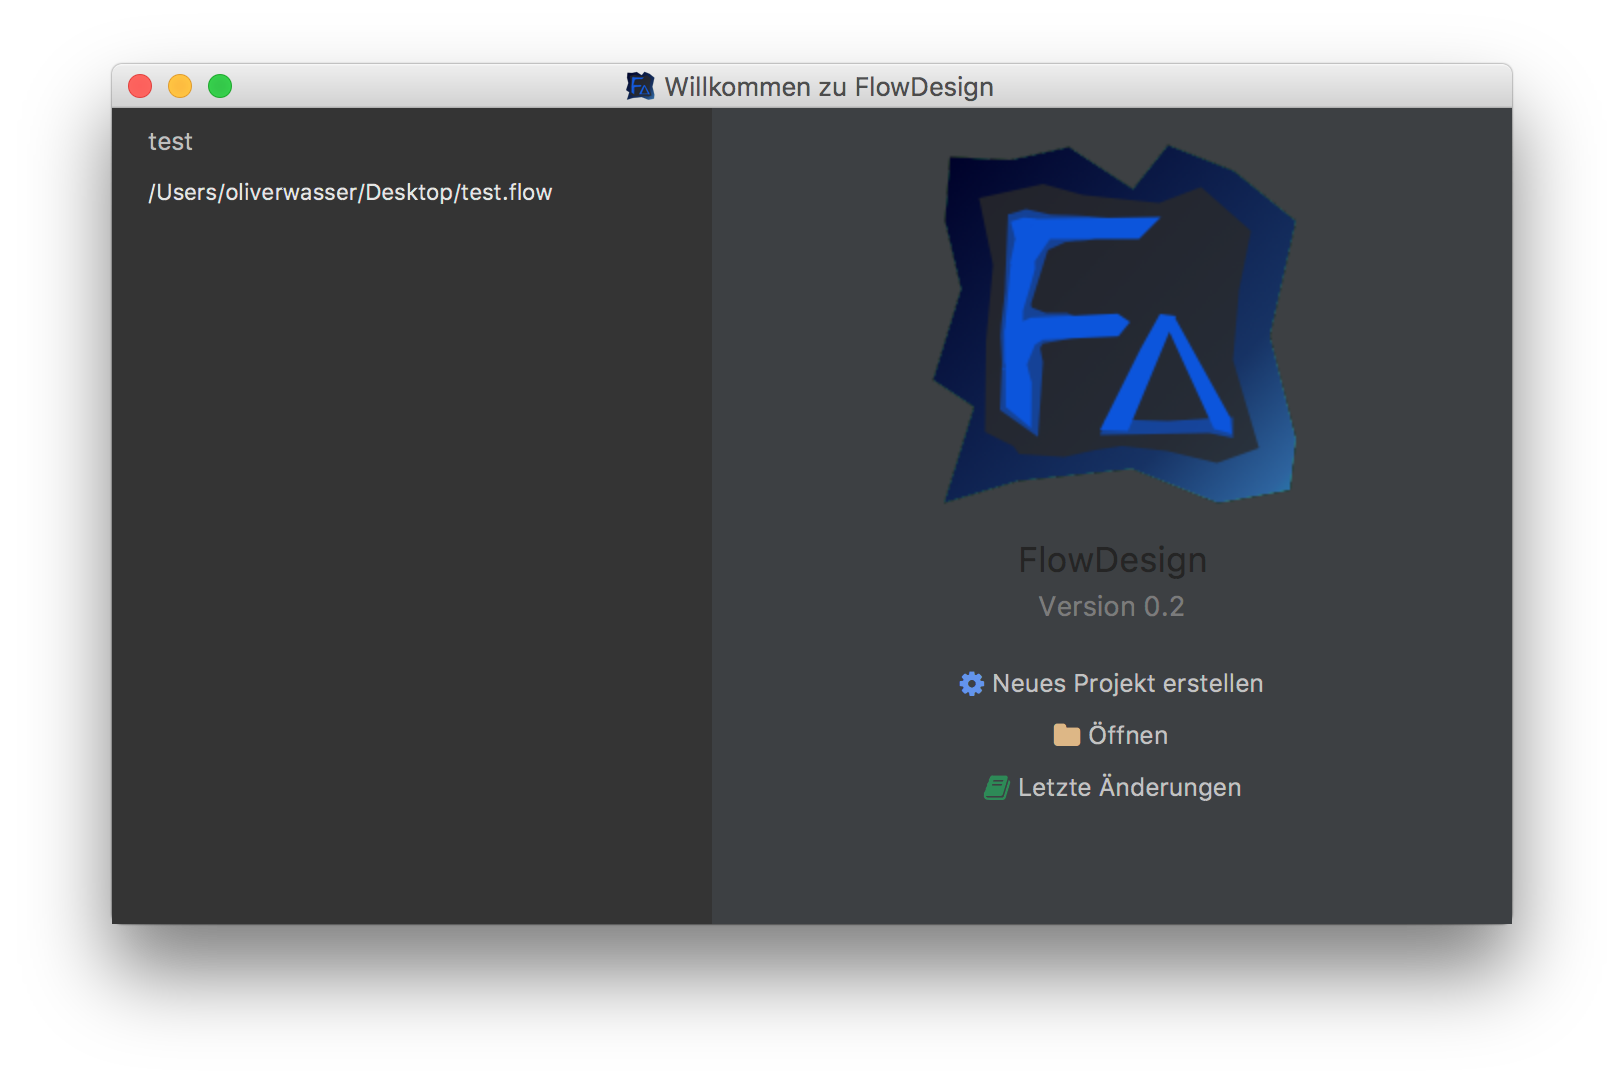
\includegraphics[width=1.0\textwidth]{Auswahlfenster.png}
	\caption{Auswahlfenster}
\end{figure}


\subsubsection{Öffnen eines kürzlich erstellten Projekts}
\begin{itemize}
\item Zum Öffnen eines kürzlich erstellten Projekts, wählen Sie mit einem Doppelklick das gewünschte Projekt im linken Teil des Auswahlfensters. 
\end{itemize}
\subsubsection{Öffnen eines beliebigen Projekts}
\begin{itemize}
\item Zum Hinzufügen eines anderen bestehenden Projektes, wählen Sie mit einem Linksklick ''Öffnen''. Es erscheint ein Fenster zur Auswahl des Dateipfades. Wählen Sie nun das gewünschte Projekt als ''.flow'' Datei aus und bestätigen Sie anschließend mit ''Open''. 
\end{itemize}
\subsubsection{Erstellen eines neuen Projekts}
\begin{itemize}
\item Zum Erstellen eines neuen Projektes, drücken Sie "Neues Projekt erstellen". Im folgenden Fenster tragen Sie einen Name und Speicherort für Ihr Projekt ein. Bestätigen Sie mit ''Ok''.  
\end{itemize}

\subsection{Projektfenster}
\subsubsection{Menüleiste}
\begin{figure}[h!]
	\centering
	
\includegraphics[width=1.0\textwidth]{Leiste.png}
	\caption{Menüleiste unter macOS}
\end{figure}
\begin{itemize}
\item Die Menüleiste enthält die Auswahlpunkte ''Datei'', ''Bearbeiten'', ''Aktion'', ''Diagramm'' und ''Hilfe''.
\item Die für die einzelnen Aktionen nötigen Shortcuts werden Ihnen jeweils zugehörig in der Menüleiste angezeigt. 

\begin{figure}[h!]
	\centering
	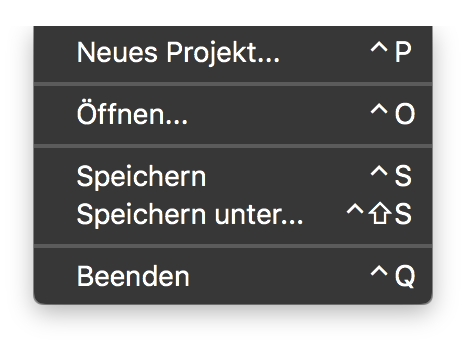
\includegraphics[width=.4\textwidth]{Leiste_Datei.png}
	\caption{Menüleiste - ''Datei''}
\end{figure}

\item Unter ''Datei'' ist es Ihnen möglich ein anderes Projekt zu öffnen, das aktuelle Projekt zu speichern oder mit ''Speichern unter'' eine neue Kopie unter einem beliebigen Pfad abzulegen.

\begin{figure}[h!]
	\centering
	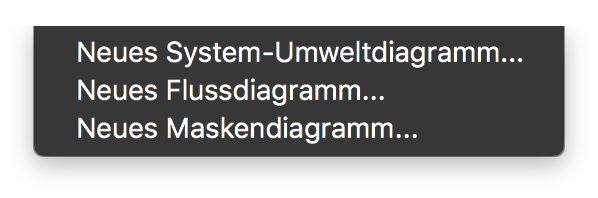
\includegraphics[width=.4\textwidth]{Leiste_Bearbeiten.png}
	\caption{Menüleiste - ''Bearbeiten''}
\end{figure}

\item Unter ''Bearbeiten'' haben Sie die Möglichkeit neue Diagramme jedes Typen zu erstellen.

\begin{figure}[h!]
	\centering
	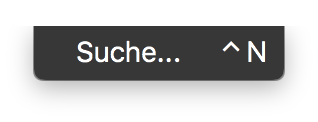
\includegraphics[width=.4\textwidth]{Leiste_Aktion.png}
	\caption{Menüleiste - ''Aktion''}
\end{figure}

\item ''Aktion'' enthält die Suche nach Diagramme. Diese kann ebenfalls mit dem Lupensymbol in der oberen rechten Ecke des Programmes abgerufen werden.

\begin{figure}[h!]
	\centering
	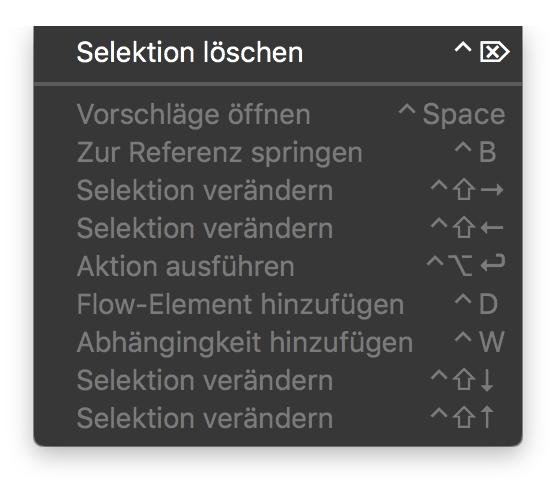
\includegraphics[width=.4\textwidth]{Leiste_Diagram.png}
	\caption{Menüleiste - ''Diagram''}
\end{figure}

\item  Unter ''Diagramm'' finden Sie sämtliche Optionen die das intelligente Arbeiten mit Diagrammen betrifft. Dazu gehört der Quick-Jump in verlinkte Diagramme oder das Hinzufügen von Abhängigkeiten.

\begin{figure}[h!]
	\centering
	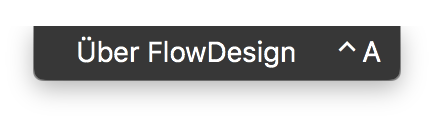
\includegraphics[width=.4\textwidth]{Leiste_Hilfe.png}
	\caption{Menüleiste - ''Hilfe''}
\end{figure}

\item Wählen Sie ''Hilfe'', um Informationen über den aktuellen Programmbuild zu erhalten.
\end{itemize}

\subsubsection{Projektbaum und Anlegen neuer Diagramme}

\begin{figure}[h!]
	\centering
	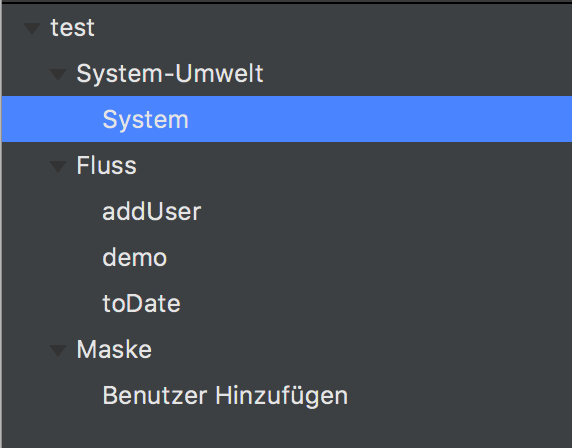
\includegraphics[width=.4\textwidth]{Projektbaum.png}
	\caption{Projektbaum}
\end{figure}

\begin{itemize}
\item Der Projektbaum befindet sich im Programm auf der linken Seite.
\item In der obersten Zeile finden Sie Ihren zuvor gewählten Projektnamen wieder, gefolgt von den drei Diagrammtypen 'System-Umwelt', ‘Fluss‘ und ‘Maske‘. Sie können beliebig viele Diagramme eines Typs erstellen.

\begin{figure}[h!]
	\centering
	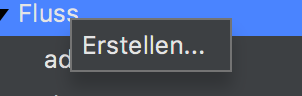
\includegraphics[width=.4\textwidth]{Projektbaum_Erstellen.png}
	\caption{Projektbaum - Erstellen}
\end{figure}

\item Um ein neues Diagramm zu erstellen, drücken Sie mit der rechten Maustaste auf den gewünschten Diagrammtyp. Wählen Sie nun ‘Erstellen' und vergeben Sie einen Namen, beachten Sie dabei das ein Name nur einmalig vergeben werden kann. 

\begin{figure}[h!]
	\centering
	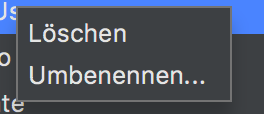
\includegraphics[width=.4\textwidth]{Projektbaum_Bearbeiten.png}
	\caption{Projektbaum - Bearbeiten}
\end{figure}

\item Um bereits erstellte Diagramme zu löschen oder umzubenennen, drücken Sie mit der rechten Maustaste auf das gewünschte Diagramm und wählen Sie die Änderung welche Sie vornehmen möchten.
\end{itemize}

\subsubsection{Zeichenfläche}
\subsubsection{Ändern des Programmdesigns}

